\section{Aligned and unaligned tilings of polyforms}
\label{sec:align}

The proof that the hat polykite is aperiodic
involves a case analysis for ways of surrounding a copy of that tile,
and that case analysis in turn involves considering possibilities for
how an individual kite in a copy of the hat polykite could fill a
particular kite on an underlying $[3.4.6.4]$ Laves tiling.  By itself
a proof founded on such a case analysis shows the absence of
periodic tilings only when all tiles are \textit{aligned} to the same 
underlying $[3.4.6.4]$ Laves tiling.  This argument leaves open the
possibility that polykites might be able to tile periodically if they
may be translated, rotated and reflected without regard to the underlying grid.
Here we
provide the necessary justification that it is sufficient to consider
aligned tilings: for classes of polyforms that include
polykites, if a tile admits a periodic tiling then it also admits one
that is aligned (in a suitable precisely defined sense); the same is
also shown for some other tiling properties such as ``isohedral'' in
place of ``periodic'', although for the purposes of the main result of
the paper, this fact is needed only for the ``periodic'' case (in which case
the result and proof are slightly simpler).  We further show that the
hat in particular does not admit any unaligned tilings.

In principle, the same issue arises for polyominoes and polyiamonds.
However, the only unaligned tilings by congruent squares consist of
parallel rows of squares slid relative to each other
(Figure~\ref{fig:slidsquares}), and much the same applies to tilings
by congruent equilateral triangles (Figure~\ref{fig:slidtriangles}),
and so it is clear that no interesting examples of unaligned tilings
by polyominoes or polyiamonds can arise.
However, kites can form nontrivial unaligned tilings such as that of
Figure~\ref{fig:slidhextrikites}, and so there is genuinely something to
be proved here, less obvious than it is for polyominoes and
polyiamonds.

\begin{figure}[htp!]
\begin{center}
\begin{tikzpicture}[x=1cm,y=1cm]
  \drawsquare{0}{0};
  \drawsquare{1}{0};
  \drawsquare{2}{0};
  \drawsquare{3}{0};
  \drawsquare{4}{0};
  \drawsquare{5}{0};
  \drawsquare{0.2}{1};
  \drawsquare{1.2}{1};
  \drawsquare{2.2}{1};
  \drawsquare{3.2}{1};
  \drawsquare{4.2}{1};
  \drawsquare{-0.1}{2};
  \drawsquare{0.9}{2};
  \drawsquare{1.9}{2};
  \drawsquare{2.9}{2};
  \drawsquare{3.9}{2};
  \drawsquare{4.9}{2};
\end{tikzpicture}
\end{center}
\caption{Sliding rows of squares}
\label{fig:slidsquares}
\end{figure}

\begin{figure}[htp!]
\begin{center}
\begin{tikzpicture}[x=1cm,y=1cm]
  \drawtriangle{0}{0}{0};
  \drawtriangle{-60}{0}{1};
  \drawtriangle{0}{0}{1};
  \drawtriangle{-60}{0}{2};
  \drawtriangle{0}{0}{2};
  \drawtriangle{-60}{0}{3};
  \drawtriangle{0}{0}{3};
  \drawtriangle{-60}{0}{4};
  \drawtriangle{0}{0}{4};
  \drawtriangle{0}{1}{-0.7};
  \drawtriangle{-60}{1}{0.3};
  \drawtriangle{0}{1}{0.3};
  \drawtriangle{-60}{1}{1.3};
  \drawtriangle{0}{1}{1.3};
  \drawtriangle{-60}{1}{2.3};
  \drawtriangle{0}{1}{2.3};
  \drawtriangle{-60}{1}{3.3};
  \drawtriangle{0}{1}{3.3};
  \drawtriangle{0}{2}{-1.3};
  \drawtriangle{-60}{2}{-0.3};
  \drawtriangle{0}{2}{-0.3};
  \drawtriangle{-60}{2}{0.7};
  \drawtriangle{0}{2}{0.7};
  \drawtriangle{-60}{2}{1.7};
  \drawtriangle{0}{2}{1.7};
  \drawtriangle{-60}{2}{2.7};
  \drawtriangle{0}{2}{2.7};
\end{tikzpicture}
\end{center}
\caption{Sliding columns of equilateral triangles}
\label{fig:slidtriangles}
\end{figure}

\begin{figure}[htp!]
\begin{center}
\begin{tikzpicture}[x=5mm,y=5mm]
  \hexkites{0}{0}{0}{0};
  \trikites{-120}{0}{0}{0}{0};
  \trikites{-60}{2}{-2}{0}{0};
  \trikites{0}{4}{-2}{0}{0};
  \trikites{60}{4}{0}{0}{0};
  \trikites{120}{2}{2}{0}{0};
  \trikites{180}{0}{2}{0}{0};
  \hexkites{2}{-4}{2}{0};
  \hexkites{4}{-2}{0}{2};
  \hexkites{2}{2}{-2}{2};
  \hexkites{-2}{4}{-2}{0};
  \hexkites{-4}{2}{0}{-2};
  \hexkites{-2}{-2}{2}{-2};
  \trikites{-120}{2}{-4}{2}{0};
  \trikites{-60}{6}{-4}{0}{2};
  \trikites{0}{6}{0}{-2}{2};
  \trikites{60}{2}{4}{-2}{0};
  \trikites{120}{-2}{4}{0}{-2};
  \trikites{180}{-2}{0}{2}{-2};
\end{tikzpicture}
\end{center}
\caption{Unaligned tiling of kites}
\label{fig:slidhextrikites}
\end{figure}

In order to apply the results presented here to other classes of 
polyforms such as polyaboloes,
we state the required conditions on the tiles in fairly general and
technical form.

Let $S$ be a set of real numbers that are linearly
independent over~$\mathbb{Q}$.  Let $\mathcal{P}$ be a finite set of
closed topological disk polygonal tiles, such that all the angles
of corners of tiles in~$\mathcal{P}$ are rational sub-multiples of~$\pi$,
all the lengths of sides of tiles in~$\mathcal{P}$ are integer
multiples of elements of~$S$, and such that, if a polygon
in~$\mathcal{P}$ has two or more collinear sides,
the lengths of those sides are integer multiples of the same element
of~$S$, as are the distances between their endpoints.

We now consider clusters of tiles built using copies of the polygons
in $\mathcal{P}$.  Let $\mathcal{Q}$ be a nonempty set of tiles, each
one congruent
to one of the polygons in $\mathcal{P}$, with disjoint interiors.  
The set $\mathcal{Q}$ may cover the entire plane, or just part of it.
The union of the boundaries of the tiles in $\mathcal{Q}$ decomposes
into a set of maximal line segments, rays, and infinite lines, which we will
refer to generically as \textit{segments}.  These segments are maximal
in the sense that no segment is a subset of a longer line contained in
the union of the tile boundaries.

Given one such maximal segment~$\ell$, and two tiles $A, B\in\mathcal{Q}$
(which may be identical), we say that $A$ and~$B$ are \emph{$\ell$-aligned}
if they both have sides that are subsets of~$\ell$, all sides of $A$
or~$B$ that lie in~$\ell$ have lengths that are integer multiples of
the same $s\in S$, and the distance between any endpoint of
one of those sides that lies in~$\ell$ and any other such endpoint is
also an integer multiple of~$s$.

The set $\mathcal{Q}$ naturally induces a graph whose vertices correspond
to the tiles in the set.  Two tiles $A$ and $B$ are connected by an edge
in the graph if there is a maximal segment~$\ell$ such that $A$ and $B$
are $\ell$-aligned and intersect in a line segment of positive length
that is a subset of $\ell$.
We say that $\mathcal{Q}$ is \emph{weakly aligned} if this graph is 
connected.  We say that it is \emph{strongly aligned} if it is weakly 
aligned and, for every maximal segment~$\ell$ determined by $\mathcal{Q}$,
and all tiles $A$ and~$B$ that have sides
lying in~$\ell$, $A$ and~$B$ are $\ell$-aligned.  We say that
\emph{$\mathcal{P}$ has the alignment property for side
lengths~$S$} if every weakly aligned set is strongly
aligned.  Here we drop the qualifiers ``strongly'' and ``weakly'' and refer 
to $\mathcal{Q}$, given the combination
of~$\mathcal{P}$ and~$S$, simply as \emph{aligned}.

\begin{lemma}
Any finite set of polykites, where the underlying kites have side
lengths $1$ and~$\sqrt{3}$, has the alignment property for side
lengths $\{1,\sqrt{3}\}$.
\end{lemma}

\begin{proof}
In the Laves tiling $[3.4.6.4]$, subdivide each kite into
$30^\circ$--$60^\circ$--$90^\circ$ triangles as shown in
Figure~\ref{fig:kitedecomp24}, forming a $[4.6.12]$
Laves tiling.  Furthermore, if a kite congruent to
one of those from the original $[3.4.6.4]$ adjoins edge-to-edge a kite
that is a union of triangles from that $[4.6.12]$ tiling, then it too
is such a union.  Thus all polykites
in any weakly aligned set are unions of tiles from the same $[4.6.12]$
tiling.  On any line in the union of the boundaries of the tiles from
$[4.6.12]$ that contains sides with rational length, sides of such
kites can only be at integer offsets from each other, and on the other
lines (containing sides with length a rational multiple
of~$\sqrt{3}$), sides of such kites can only be at offsets from each
other that are integer multiples of~$\sqrt{3}$ (both of these facts
follow from consideration of which vertices have the correct angles to
form a corner of such a kite).  So every weakly aligned set is
strongly aligned.
\end{proof}

\begin{figure}[htp!]
\begin{center}
\begin{tikzpicture}[x=1cm,y=1cm]
  \draw \vcoords{0}{0} -- \vcoords{3}{-3} -- \vcoords{6}{0} --
    \vcoords{0}{3} -- cycle;
  \draw \vcoords{0}{0} -- \vcoords{6}{0};
  \draw \vcoords{3}{-3} -- \vcoords{3}{1.5};
  \draw \vcoords{0}{3} -- \vcoords{4.5}{-1.5};
  \draw \vcoords{3}{-3} -- \vcoords{0}{3};
  \draw \vcoords{4}{-2} -- \vcoords{2}{2};
  \draw \vcoords{5}{-1} -- \vcoords{4}{1};
  \draw \vcoords{0}{0} -- \vcoords{2}{2};
  \draw \vcoords{1.5}{-1.5} -- \vcoords{4}{1};
  \draw \vcoords{0}{0} -- \vcoords{4}{-2};
  \draw \vcoords{0}{1.5} -- \vcoords{5}{-1};
\end{tikzpicture}
\end{center}
\caption{Decomposition of a kite into $24$~triangles}
\label{fig:kitedecomp24}
\end{figure}

We now consider $\mathcal{P}$ that has the alignment property for side
lengths~$S$, and proceed to showing that, in an appropriate
sense, only aligned tilings need to be considered.  Note that for
polykites, at this point ``aligned'' means only that the kites adjoin
edge-to-edge, which is weaker than all tiles coming from the same
underlying $[3.4.6.4]$ tiling; there will be further lemmas specific
to polykites to show that we need only consider tilings where all
tiles come from the same underlying $[3.4.6.4]$.

The alignment property implies that the tiles of any tiling can be
partitioned into strongly aligned sets such that for any maximal line
segment~$\ell$ in the union of the boundaries of the tiles, and any
two tiles in different sets that have sides sharing a segment of
positive length lying on~$\ell$, those two tiles are not
$\ell$-aligned.  We refer to these as the \emph{aligned components} of
the tiling.  Each aligned component is a connected set (possibly
unbounded), with connected interior.

Suppose $\mathcal{C}$ is an aligned component in a tiling, and
$\mathcal{D}$~is a connected component of the complement
of~$\mathcal{C}$ ($\mathcal{D}$ might be the interior of another
aligned component, or might be the interior of the union of more than
one aligned component).  The boundary of~$\mathcal{D}$ consists of a single
polygonal curve, either closed or infinite, and as with any other
polygon we may speak of its corners and sides.  Furthermore, that
curve cannot pass through the same point more than once; if it did,
either $\mathcal{D}$ (an open set) would not be connected, or
$\mathcal{C}$ would not have connected interior.

Consider traversing the boundary of~$\mathcal{D}$; note that
$\mathcal{D}$ always lies on the same side of the boundary during that
traversal.  When the traversal
encounters a corner, say that corner is convex if an open line segment
between two points on the curve sufficiently close to that corner but
on opposite sides of it is entirely within~$\mathcal{D}$.

When the boundary of~$\mathcal{D}$ is a closed curve, we must also
initially allow for $\mathcal{D}$ being inside that curve (a hole
in~$\mathcal{C}$) or outside (in which case $\mathcal{C}$ is
bounded).  The following lemma shows that the first of those cases
cannot occur, since if $\mathcal{D}$ is inside the curve it must have
at least three convex corners.

\begin{lemma}
The boundary of~$\mathcal{D}$ has no convex corners if it is a closed
curve (so in that case $\mathcal{C}$ must be a bounded convex set),
and at most one convex corner if it is an infinite curve.
\end{lemma}

\begin{proof}
If we consider any finite side of the
boundary of~$\mathcal{D}$, lying in some maximal line segment~$\ell$,
all the tiles lying on the other side of the side from~$\mathcal{D}$
are not $\ell$-aligned with any of those in~$\mathcal{D}$, meaning
that at least one of the two corners at the ends of that side lies in
the middle of a side of such a tile.  If $v$~is a convex corner, and
$v_1$, $v_2$, \ldots\ are successive vertices traversing the boundary
curve in one direction from~$v$, then we conclude that $v_1$~lies in
the middle of a side of a tile on the same line as~$vv_1$, then that
$v_2$~lies in the middle of a side of a tile on the same line
as~$v_1v_2$, and so on.  This results in a contradiction if we
encounter another convex corner (see Figure~\ref{fig:twoconvex} for an
illustration), or encounter $v$~again on a closed curve (see
Figure~\ref{fig:closedconvex}).
\end{proof}

\begin{figure}[htp!]
\begin{center}
\begin{tikzpicture}[x=1cm,y=1cm]
  \draw (0,0) -- (1,0) -- (2,1) -- (3,1) -- (4,0) -- (5,0);
  \draw (3,1) -- (2.5,1.5);
  \draw (2,1) -- (1.5,1);
  \draw (4.2,0.2) node {$v$};
  \draw (3.2,1.2) node {$v_1$};
  \draw (1.8,1.2) node {$v_2$};
\end{tikzpicture}
\end{center}
\caption{Boundary curve with two convex corners}
\label{fig:twoconvex}
\end{figure}

\begin{figure}[htp!]
\begin{center}
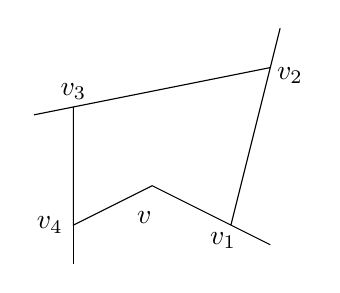
\begin{tikzpicture}[x=1cm,y=1cm]
  \draw (0,0) -- (1,0.5) -- (2,0) -- (2.5,2) -- (0,1.5) -- cycle;
  \draw (2,0) -- (2.5,-0.25);
  \draw (2.5,2) -- (2.625,2.5);
  \draw (0,1.5) -- (-0.5,1.4);
  \draw (0,0) -- (0,-0.5);
  \draw (0.9,0.1) node {$v$};
  \draw (1.9,-0.2) node {$v_1$};
  \draw (2.75,1.9) node {$v_2$};
  \draw (0,1.7) node {$v_3$};
  \draw (-0.3,0) node {$v_4$};
\end{tikzpicture}
\end{center}
\caption{Closed boundary curve with a convex corner}
\label{fig:closedconvex}
\end{figure}

Now we need to list the tiling properties for which our argument says
we do not need to consider unaligned tilings.  Let $H$ be one of the
following predicates on a tiling~$\mathcal{T}$; here, $k$~may be any
positive integer.

\begin{itemize}
\item $\mathcal{T}$ is a tiling (the trivial predicate).
\item $\mathcal{T}$ is a strongly periodic tiling.
\item $\mathcal{T}$ is a weakly periodic tiling.
\item $\mathcal{T}$ is a tiling with at most $k$~orbits of tiles
  under the action of its symmetry group.
\item $\mathcal{T}$ is an isohedral tiling by $180^\circ$ rotation.
\item $\mathcal{T}$ is an isohedral tiling by translation.
\end{itemize}

\begin{lemma}
\label{lemma:align}
If $\mathcal{P}$ admits a tiling with property~$H$, it admits an
aligned tiling with property~$H$.
\end{lemma}

\begin{proof}
Consider a tiling~$\mathcal{T}$ with property~$H$ and look at the
forms aligned components take in that tiling.  By the previous lemma,
such components must be simply connected; either bounded, or unbounded
and with each boundary curve having at most one convex corner (in the
sense defined above, i.e., convex considered as a corner of a
connected component of the complement of the aligned component).

If such a component is the whole plane, the tiling is aligned and we
are done.  If it is a half-plane, form an aligned tiling of that
component and its reflection, and that tiling has property~$H$ (which
can only be the trivial property or ``weakly periodic'' in that case).
If it is a strip infinite in both directions, with straight lines as
its boundaries on both sides, repeat that strip by translation if
there is such a tiling that is aligned, and otherwise repeat it by
$180^\circ$ rotation; by considering separately for each possible
predicate~$H$, the resulting aligned tiling has property~$H$.

Otherwise, if there is any unbounded component, it does not have a
translation as a symmetry and $H$~is the trivial predicate.  If an
unbounded component contains balls of radius~$R$ for all~$R$, there
are aligned tilings of arbitrarily large regions of the plane, and so
of the whole plane.  The only way an unbounded component can avoid
containing such balls (given that each boundary curve has at most one
convex corner and all angles are rational sub-multiples of~$\pi$, which
implies that all boundary curves end in rays in finitely many
directions) is for it to include a semi-infinite strip (bounded on
either side by rays).  But there are only finitely many ways for
aligned tiles to cross the width of the strip at any point, so tiling
a semi-infinite strip implies the existence of a periodic aligned
tiling of an infinite strip, and thus a periodic aligned tiling of the
whole plane.

It remains to consider the case where there is no unbounded component.
If some component is a triangle or a quadrilateral, tiling that by
$180^\circ$~rotation yields an aligned tiling of the whole plane,
which must have property~$H$ (if property~$H$ is `isohedral tiling by
translation', this case cannot occur; a component could be an infinite
strip, but not a single parallelogram).  If components contain
unbounded balls, the tiling has no translation as a symmetry and
aligned tilings of arbitrarily large regions of the plane imply
aligned tilings of the whole plane.  If components do not contain
unbounded balls but also are not contained in bounded balls (i.e.,
they are of unbounded size in one direction only), they must have
pairs of opposite parallel sides, of unbounded length but a bounded
distance apart; the tiling is at most weakly periodic, and the same
argument as for components including a semi-infinite strip applies
since there are only finitely many possible distances between those
opposite parallel sides.

Otherwise, all components are convex polygons of bounded size with at
least five sides; we will show this case leads to a contradiction.  
Observe that every
vertex of the induced tiling by these polygons lies in the middle of a
side of one of the polygons and has degree exactly~$3$.
If a vertex does not lie in the middle of a side, or has
degree $4$ or more, there is a vertex~$v$ of a polygon~$P$, either not
in the middle of a side or in the middle of a side that is not
collinear with either of the sides $vv_1$ and $vv_2$ of~$P$ next
to~$v$, and the same argument that excluded convex corners on a closed
curve earlier serves to exclude this possibility as well.

We now apply Euler's theorem for plane maps.  Suppose, for some
sufficiently large~$R$, a ball of radius~$R$ contains $t_k$ components
that are $k$-gons (where $\sum_k t_k = \Omega(R^2)$).  A vertex of the
tiling is incident with two corners of tiles and a point in the middle
of a side, so there are $\sum_k k t_k / 2 + O(R)$ vertices in that
ball.  The number of sides of edges in the tiling in that ball (i.e.,
twice the number of edges) is $\sum_k \frac{3}{2}k t_k + O(R)$, since
there are $\sum_k k t_k + O(R)$ sides of polygons, and each vertex is
in the middle of a side so serves to increase the number of sides of
edges by~$1$.  But now $\sum_k t_k + \sum_k k t_k / 2 = \sum_k
\frac{3}{4}k t_k + O(R)$, so $\sum_k t_k = \sum_k k t_k / 4 + O(R)$.
Since all $k \ge 5$, we have $\sum_k k t_k / 4 \ge \sum_k \frac{5}{4}
t_k$, contradicting that equality.
\end{proof}

Now we strengthen this lemma to a stricter notion of aligned tilings by
polykites, by considering what edge-to-edge tilings by the monokite
are possible.

\begin{lemma}
The only edge-to-edge tilings by the monokite are (a) the tiling
resulting from a $180^\circ$~rotation about the midpoint of each side
(Figure~\ref{fig:kite180tiling}), and (b) tilings composed of rows of
equilateral triangles each composed of three kites, where some of
those rows may be slid relative to each other (by the length of the
long side of the kite) so they are no longer aligned as in the Laves
tiling.
\end{lemma}

\begin{figure}[htp!]
\begin{center}
\begin{tikzpicture}[x=2mm,y=2mm]
  \threekite{0}{0}{0}{};
  \threekite{180}{-1.5}{0}{};
  \threekite{0}{1}{1}{};
  \threekite{180}{-0.5}{1}{};
  \threekite{0}{2}{2}{};
  \threekite{180}{0.5}{2}{};
  \threekite{0}{1.5}{-1.5}{};
  \threekite{180}{0}{-1.5}{};
  \threekite{0}{2.5}{-0.5}{};
  \threekite{180}{1}{-0.5}{};
  \threekite{0}{3.5}{0.5}{};
  \threekite{180}{2}{0.5}{};
  \threekite{0}{3}{-3}{};
  \threekite{180}{1.5}{-3}{};
  \threekite{0}{4}{-2}{};
  \threekite{180}{2.5}{-2}{};
  \threekite{0}{5}{-1}{};
  \threekite{180}{3.5}{-1}{};
\end{tikzpicture}
\end{center}
\caption{$180^\circ$ tiling by kites}
\label{fig:kite180tiling}
\end{figure}

\begin{proof}
There are exactly two possible vertex figures in an edge-to-edge
tiling by the monokite that do not appear in the Laves tiling: one
with angles of $90^\circ$, $120^\circ$, $90^\circ$, and $60^\circ$ in
that order (Figure~\ref{fig:kite180vertex}), and one with angles of
$90^\circ$, $90^\circ$, $60^\circ$, $60^\circ$, and $60^\circ$ in that
order (Figure~\ref{fig:kiteslidvertex}).  If the first one occurs in a
tiling, successive surrounding tiles are forced (in the order
numbered) that force all neighbouring vertices, and so all vertices,
to have that vertex figure.  If the other one occurs in a tiling,
successive surrounding tiles are forced (in the order numbered, taking
into account that the first vertex figure cannot appear anywhere in
the tiling) that force two neighbouring vertices to have that vertex
figure, and thus force two rows of equilateral triangles, slid
relative to each other, and then the only possibilities on either side
of such a row are another such row in either of two positions.
\end{proof}

\begin{figure}[htp!]
\begin{center}
\begin{tikzpicture}[x=2mm,y=2mm]
  \threekite{0}{0}{0}{};
  \threekite{180}{-1.5}{0}{};
  \threekite{0}{1}{1}{};
  \threekite{180}{0}{-1.5}{};
  \threekite{180}{1}{-0.5}{1};
  \threekite{0}{2.5}{-0.5}{2};
  \threekite{180}{1.5}{-3}{3};
  \threekite{0}{1.5}{-1.5}{4};
  \threekite{180}{-1}{-2.5}{5};
  \threekite{0}{-1}{-1}{6};
  \threekite{180}{-2.5}{-1}{7};
  \threekite{0}{-1.5}{1.5}{8};
  \threekite{0}{-0.5}{2.5}{9};
  \threekite{180}{-3}{1.5}{10};
  \threekite{180}{-0.5}{1}{11};
  \threekite{0}{2}{2}{12};
  \markpt{2}{0};
\end{tikzpicture}
\end{center}
\caption{Vertex with angles of $90^\circ$, $120^\circ$, $90^\circ$, and
  $60^\circ$ in that order}
\label{fig:kite180vertex}
\end{figure}

\begin{figure}[htp!]
\begin{center}
\begin{tikzpicture}[x=2mm,y=2mm]
  \threekite{0}{0}{0}{};
  \threekite{60}{0}{0}{};
  \threekite{120}{0}{0}{};
  \threekite{180}{-1.5}{0}{};
  \threekite{-60}{1.5}{0}{};
  \threekite{60}{-1.5}{3}{1};
  \threekite{120}{-3}{0}{2};
  \threekite{-120}{0}{-3}{3};
  \threekite{180}{0}{-3}{4};
  \threekite{-60}{3}{-3}{5};
  \threekite{-120}{3}{-3}{6};
  \threekite{0}{3}{0}{7};
  \threekite{-120}{-1.5}{0}{8};
  \threekite{-60}{-1.5}{0}{9};
  \threekite{-120}{1.5}{0}{10};
  \threekite{180}{1.5}{0}{11};
  \markpt{2}{0};
\end{tikzpicture}
\end{center}
\caption{Vertex with angles of $90^\circ$, $90^\circ$, $60^\circ$,
  $60^\circ$, and $60^\circ$ in that order}
\label{fig:kiteslidvertex}
\end{figure}

\begin{lemma}
\label{lemma:polykitealign}
If $\mathcal{P}$ is a finite set of closed topological disk polykites,
all from the same underlying Laves tiling, and $\mathcal{P}$ admits a
tiling with property~$H$, it admits a tiling with property~$H$ where
all polykites in the tiling are aligned to the same underlying Laves
tiling, except possibly when $\mathcal{P}$ contains the monokite and
$H$ is ``isohedral tiling by $180^\circ$ rotation''.
\end{lemma}

\begin{proof}
If the edge-to-edge tiling with property~$H$ (``aligned'' in the more
general sense) is the $180^\circ$ tiling by the monokite, we are done
because the monokite admits an isohedral tiling.  Otherwise, taking a
minimal block of consecutive rows of equilateral triangles filled
exactly with tiles from~$\mathcal{P}$ and translating it so as to be
aligned with the underlying Laves tiling produces a tiling with
property~$H$.
\end{proof}

\begin{lemma}
\label{lemma:tileaalign}
All tilings by the hat polykite are aligned
to an underlying $[3.4.6.4]$ Laves tiling.
\end{lemma}

\begin{proof}
Note that any maximal segment in the union of the boundaries of tiles in such
a tiling can contain no more than two sides of tiles, since any
$90^\circ$~angle is adjacent on either side to angles greater
than~$90^\circ$.  In particular, there are no infinite rays contained
in the union of the boundaries of tiles.

This constraint immediately excludes the case of aligned tilings decomposing 
into rows of equilateral triangles slid relative to each other, and no two
adjacent kites in the polykite are consistent with the
$180^\circ$~rotation tiling by the monokite.  So any tiling not
aligned with an underlying $[3.4.6.4]$ is also unaligned in the more
general sense, and we consider aligned components.  Because there are
no infinite rays among the boundaries of tiles, such aligned
components must be bounded convex sets.  The corners of those sets
must be corners of a single polykite (since any two angles of the
polykite add to at least~$180^\circ$).  But no corner of the polykite
can be a corner of a convex set tiled by the polykite: four have
reflex angles, seven are adjacent to a reflex angle, and for the
remaining two, extending one of the sides from that vertex cuts off a
region too small to be filled by polykites
(Figure~\ref{fig:polykiteconvex}).
\end{proof}

\begin{figure}[htp!]
\begin{center}
\begin{tikzpicture}[x=5mm,y=5mm]
  \draw[\colextside,ultra thick] \vcoords{0}{0} -- \vcoords{4}{-4};
  \draw[\colextside,ultra thick] \vcoords{6}{-5} -- \vcoords{6}{-2};
  \tileA{0}{0}{0}{};
  \markpt{0}{0};
  \markpt{6}{-5};
\end{tikzpicture}
\end{center}
\caption{Extending a side of the polykite from either vertex that is
  neither a reflex angle nor adjacent to one}
\label{fig:polykiteconvex}
\end{figure}
